%
% slides.tex -- Slides für Woche 4
% 
\section{Separation}

\begin{frame}
\frametitle{Zusammenfassung: Separation}
\begin{enumerate}
\item Koordinaten: m"ussen zu Gebietsgrenzen passen
\item Separationsansatz: 
\begin{align*}
&\text{meistens:}&u(x,y)&=X(x)\cdot Y(y)\\
&\text{manchmal:}&u(x,y)&=X(x)+Y(y)
\end{align*}
\item Einsetzen und Variablen trennen
\[
\text{nur $x$} = \text{nur y}\quad\Rightarrow\quad \text{beide konstant $=\mu$}
\]
$\Rightarrow$ Eigenwertproblem
\item Nullrandbedingungen legen $\mu$ fest: $\mu_1$, $\mu_2$,
$\mu_3,\dots,\mu_n,\dots$
\item Teill"osungen $u_n(x,y)=X_n(x)\cdot Y_n(y)$  zu jedem $\mu_n$
\item "Uberlagerung (nur f"ur lineare PDGL)
\[
u(x,y)=\sum_n a_nu_n(x,y)
\]
\item Koeffizienten $a_n$ aus verbleibenden Randbedingungen
\end{enumerate}
\end{frame}

\begin{frame}
\section{Tsunami}
\frametitle{Sendai-Erdbeben 2011}
\begin{center}
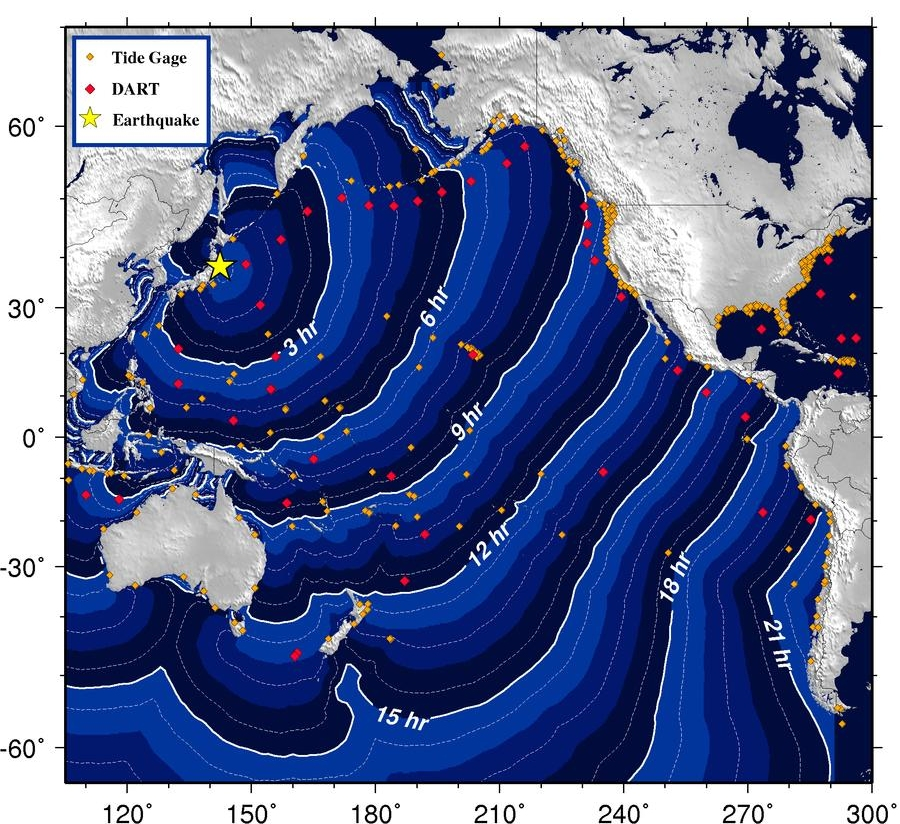
\includegraphics[width=0.85\hsize]{../../skript/graphics/sendainoaa.jpg}
\end{center}
\end{frame}

\begin{frame}
\frametitle{Tsunami}
{\bf Wellengleichung} auf der Kugeloberfl"ache:
\[
\frac{1}{c^2}\frac{\partial^2u}{\partial t^2}
=
\Delta u
\]
{\bf Kugel-Koordinaten:} $(r,\vartheta,\varphi)$,
d.~h.~$u(t,r,\vartheta,\varphi)$

\medskip

{\bf Laplaceoperator:}
\[
\Delta = \frac{1}{r^2}\frac{\partial}{\partial r}r^2\frac{\partial}{\partial r}
+
\frac{1}{r^2\sin\vartheta}\frac{\partial}{\partial\vartheta}\sin\vartheta\frac{\partial}{\partial\vartheta}
+
\frac1{r^2\sin^2\vartheta}\frac{\partial^2}{\partial\varphi^2}
\]
{\bf Symmetrie:}
\begin{enumerate}
\item Unabh"angig von $r$, d.~h.~$r=1$
\item Rotationssymmetrie um Epizentrum
\end{enumerate}

{\bf Randbedingungen:}
\begin{align*}
\frac{\partial u}{\partial\vartheta}(t,0)&=0
&
u(0,\vartheta)&=F(\vartheta)
\\
\frac{\partial u}{\partial\vartheta}(t,\pi)&=0
&
\frac{\partial u}{\partial t}(0,\vartheta)&=G(\vartheta)
\end{align*}

\end{frame}

\begin{frame}
\frametitle{L"osung}
\begin{enumerate}%[<+->]
\item Ansatz: $u(t,\vartheta)=T(t)\cdot \Theta(\vartheta)$
\item Separation:
\[
\frac{1}{c^2}\frac{T''(t)}{T(t)}
=
m
=
\frac{1}{\Theta(\vartheta)\sin\vartheta}\frac{\partial}{\partial\vartheta}\sin\vartheta
\Theta'(\vartheta)
\]
\item L"osung f"ur $T(t)$:
\[
T_m(t)=\cos\sqrt{-m}t
\qquad\text{oder}\qquad
T_m(t)=\sin\sqrt{-m}t
\]
\item L"osung f"ur $\Theta(\vartheta)$: Polynom $P_k(\cos\vartheta)$,
$m_k=-k(k+1)$
\item Allgemeine L"osung: "Uberlagerung
\[
u(t,\vartheta)=
\sum_{k=0}^\infty
(a_k\cos\sqrt{-m_k}t+b_k\sin\sqrt{-m_k}t)P_k(\cos\vartheta)
\]
\item Anfangsbedingungen: Fouriertheorie f"ur Legendre-Polynome
\end{enumerate}

\end{frame}

%\begin{frame}
%\frametitle{L"osung $\Theta(\vartheta)$}
%\begin{enumerate}
%\item Substition $z=\cos\vartheta$, $y(z)=\Theta(\cos\vartheta)$
%\item Legendre-Differentialgleichung:
%\[
%\frac{d}{dz}(1-z^2)\frac{d}{dz}y(z) =my(z).
%\]
%\item Fall $m=0$:
%\[
%y(z)=\frac{C}2\frac{1+z}{1-z}+D
%\]
%\item Allgemeiner Fall: Legendre-Polynome $P_k^l(z)$, aber nur
%f"ur $m_k=-k(k+1)$, $k\in\mathbb N$ und $l=0,1,\dots,n$.
%Wir brauchen nur $l=0$.
%\end{enumerate}
%\end{frame}
%
%\begin{frame}
%\frametitle{Approximation}
%\begin{center}
%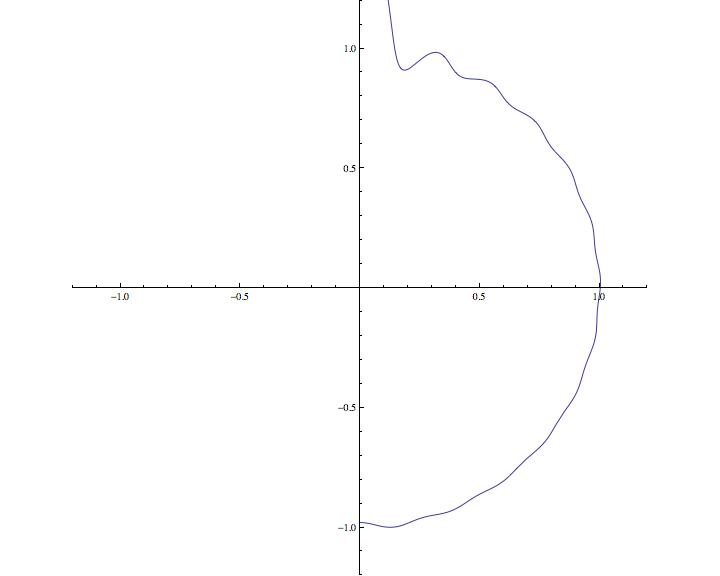
\includegraphics[width=0.9\hsize]{../../skript/graphics/tsunami0.jpg}
%\end{center}
%\end{frame}
%
%\begin{frame}
%\frametitle{Approximation}
%\begin{center}
%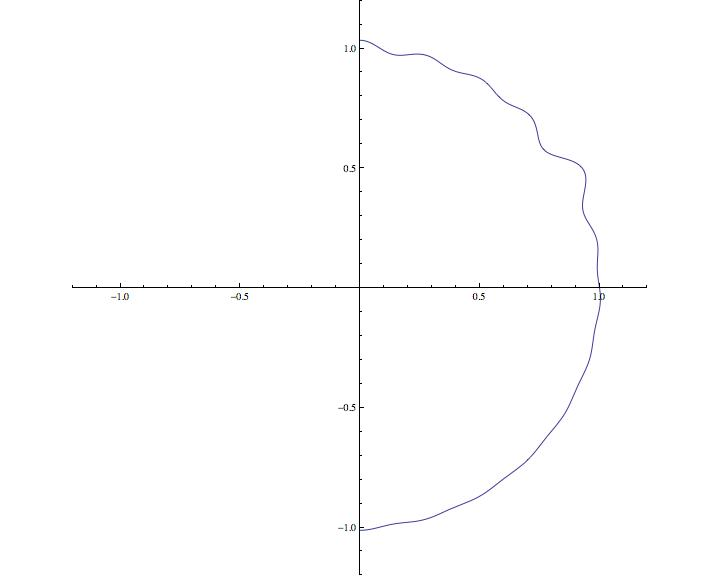
\includegraphics[width=0.9\hsize]{../../skript/graphics/tsunami50.jpg}
%\end{center}
%\end{frame}

\section{Transformation}

\begin{frame}
\frametitle{Differentialgleichung}

Wellengleichung:
\[
\frac{1}{c^2}
\frac{\partial^2 u}{\partial t^2}
=
\frac{\partial^2 u}{\partial x^2},
\]
Gebiet:
\[
\Omega = (0,\pi)\times \mathbb R^+\to \mathbb R
\]
Randbedingungen:
\begin{align*}
u(t,   0)&= 0&u(0,x)&=f(x)\\
u(t, \pi)&= 0&\frac{\partial}{\partial t}u(0,x)&=g(x)
\end{align*}
%Fourierkoeffizienten von $f$ und $g$: $b_k^{(f)}$ und $b^{(g)}_k$

\end{frame}

\begin{frame}
\frametitle{Transformation}

{\bf Beobachtung:} Separation f"uhrt auf $\sin kx$ und $\cos kx$,
d.~h.~Fourier-Reihen.

\[
\Rightarrow
\]
\bigskip

{\bf Idee:} Fourier-Reihen von Anfang an verwenden!

\end{frame}

\begin{frame}
\frametitle{Fourier-Transformation}

Jede Funktion $f\colon [-\pi,\pi]\to\mathbb R$ kann als Fourier-Reihe
geschrieben werden:
\[
f(x)=\frac{a_0}{2}+\sum_{k=1}^\infty(a_k\cos kx+b_k\sin kx).
\]

\medskip
\pause
Dies definiert die Fouriertransformation
\medskip

\begin{align*}
{\cal F}\colon
f
&\mapsto
a_0, a_k, b_k, k> 0
\end{align*}

\end{frame}

\begin{frame}
\frametitle{Ableitungen}
$a_0$, $a_k$, $b_k$ Fourier-Koeffizienten von $f$.

\[\Rightarrow\]

Fourierkoeffizienten der Ableitung nach $x$
\begin{align*}
f'(x)&=\sum_{k=1}^\infty (-ka_k\sin kx+kb_k\cos kx)\\
f''(x)&=\sum_{k=1}^\infty (-k^2a_k\cos kx-k^2b_k\sin kx)
\end{align*}
Ableitungsoperator f"ur Fourierkoeffizienten:
\begin{align*}
a_k&\mapsto -k^2a_k\\
b_k&\mapsto -k^2b_k\\
\end{align*}
\end{frame}

\begin{frame}
\frametitle{Funktion von $x$ und $t$}

$u$ eine Funktion von $x$ und $t$:
\[
u\colon (0,\pi)\times \mathbb R^+\to \mathbb R
\]
Fourierkoeffizienten h"angen von $t$ ab:
\[
u(x,t)=\frac{a_0(t)}2+\sum_{k=1}^\infty (a_k(t)\cos kx+b_k(t)\sin kx)
\]
Fourier-Transformation
\[
{\cal F}\colon
u\mapsto
a_0(t), a_k(t), b_k(t)
\]
\pause
Implizite Separation:
\begin{enumerate}[<+->]
\item Ortsabh"angigkeit in $\cos kx$ und $\sin kx$
\item Zeitabh"angigkeit in $a_k(t)$ und $b_k(t)$
\end{enumerate}

\end{frame}

\begin{frame}
\frametitle{Transformation}
Randbedingungen:
\[
a_0=0\qquad
a_k=0\;\forall k > 0
\]
Differentialgleichung:
\begin{align*}
\frac{1}{c^2}\ddot b_k(t)&= -k^2b_k(t)
\end{align*}
Anfangsbedingung:
\begin{align*}
b_k(0)&= b_k^{(f)}& \dot b_k(0)&=b_k^{(g)}
\end{align*}
{\bf Gew"ohnliche} Differentialgleichungen f"ur die Fourier-Koeffizienten
\end{frame}

\begin{frame}
\frametitle{Differentialgleichung}

Wellengleichung:
\[
\frac{1}{c^2}
\frac{\partial^2 u}{\partial t^2}
=
\frac{{\color{red}\partial^2} u}{{\color{red}\partial x^2}},
\]
Gebiet:
\[
\Omega = \mathbb R^+ \times {\color{red}(0,\pi)} \to \mathbb R
\]
Randbedingungen:
\begin{align*}
u(t,   0)&= 0&u(0,{\color{red}x})&=f({\color{red}x})\\
u(t, \pi)&= 0&\frac{\partial}{\partial t}u(0,{\color{red}x})&=g({\color{red}x})
\end{align*}
Fourierkoeffizienten von $f$ und $g$: $b_k^{(f)}$ und $b^{(g)}_k$

\end{frame}

\begin{frame}
\frametitle{Funktion von $x$ und $t$}

%$u$ eine Funktion von $x$ und $t$:
%\[
%u\colon (0,2\pi)\times \mathbb R^+\to \mathbb R
%\]
Fourierkoeffizienten h"angen von $t$ ab:
\[
u(t,x)=\frac{a_0(t)}2+\sum_{k=1}^\infty \bigl(a_k(t)\cos kx+b_k(t)\sin kx\bigr)
\]
Fourier-Transformation:
\[
{\cal F}\colon
u\mapsto
a_0(t), a_k(t), b_k(t)
\]
Implizite Separation:
\begin{enumerate}
\item Ortsabh"angigkeit in $\cos kx$ und $\sin kx$
\item Zeitabh"angigkeit in $a_k(t)$ und $b_k(t)$
\end{enumerate}

\end{frame}

\begin{frame}
\frametitle{Transformation}
Randbedingungen:
\[
a_0=0\qquad
a_k=0\;\forall k > 0
\]
Differentialgleichung:
\begin{align*}
\frac{1}{c^2}\ddot b_k(t)&= {\color{red}-k^2}b_k(t)
\end{align*}
Anfangsbedingung:
\begin{align*}
b_k(0)&= b_k^{(f)}& \dot b_k(0)&=b_k^{(g)}
\end{align*}
{\bf Gew"ohnliche} Differentialgleichungen f"ur die Fourier-Koeffizienten
\end{frame}

\begin{frame}
\frametitle{Idee}

{\bf Lineare} Transformation $\cal T$ mit folgenden Eigenschaften

\begin{align*}
u({\color{red}x},y)&&&\mapsto &&{\cal T}u(k,y)
\\
\frac{\partial u}{\partial y}&&&\mapsto&&\frac{\partial{\cal T}u}{\partial y}(k,y)
\\
\frac{{\color{red}\partial} u}{\color{red}\partial x}&&&\mapsto&&\text{{\color{red}algebraischer Ausdruck} mit $\displaystyle {\cal T}u(k,y)$}
\\
\text{PDGL}&&&\mapsto&&\text{gew"ohnliche DGL f"ur $y\mapsto {\cal T}u(k,y)$}
\\
           &&&       &&\text{algebraische Gleichung in $k$}
\\
\text{L"osung:}&&&   &&{\cal T}^{-1}({\cal T}u)(x,y)
\end{align*}
D.~h.~{\color{red}$x$-Ableitung} wird in eine {\color{red}algebraische Operation} transformiert

\end{frame}

\section{Laplace-Transformation}

\begin{frame}
\frametitle{Laplace-Transformation}
\begin{definition}
$f\colon \mathbb R^+\to\mathbb R$ hat Laplace-Transformierte
\[
{\cal L}f(s)=\int_0^\infty f(t)e^{-st}\,dt
\]
\end{definition}
\pause
\begin{center}
\begin{tabular}{>{$}c<{$}>{$\displaystyle}c<{$}}
f(t)&({\cal L}f)(s)\\
\hline
c&\frac{c\mathstrut}{s\mathstrut}\\
t^n&\frac{n!\mathstrut}{s^{n+1}\mathstrut}\\
e^{at}&\frac{1\mathstrut}{s-a\mathstrut}\\
\sin(at)&\frac{a\mathstrut}{s^2+a^2\mathstrut}\\
\cos(at)&\frac{s\mathstrut}{s^2+a^2\mathstrut}\\
\hline
\end{tabular}
\end{center}

\end{frame}

\begin{frame}
\frametitle{Ableitung}

\begin{align*}
({\cal L}f')(s)
&=
\int_0^\infty \underbrace{\mathstrut f'(t)}_{\textstyle\uparrow}\underbrace{\mathstrut e^{-st}}_{\textstyle\downarrow}\,dt
=
\underbrace{\biggl[f(t)e^{-st}\biggr]_0^\infty}_{\textstyle-f(0)}
+s\underbrace{\int_0^\infty f(t)e^{-st}\,dt}_{\textstyle({\cal L}f)(s)}
\end{align*}

\pause

\begin{center}
\begin{tabular}{>{$}l<{$}>{$\displaystyle}l<{$}}
f(t)&({\cal L}f)(s)\mathstrut\\
\hline
f'(t)&s({\cal L}f)(s)-f(0)\\
f''(t)&s^2({\cal L}f)(s)-sf(0)-f'(0)\\
\dots&\dots\\
f^{(n)}(t)&s^n({\cal L}f)(s)-s^{n-1}f(0)-s^{n-2}f'(0)-\dots - f^{(n-1)}(0)\\
\hline
\end{tabular}
\end{center}

Ziel erreicht:
\[
\text{$n$-te Ableitung}\rightarrow \text{Multiplikation mit $s^n$}
\]
\end{frame}

\begin{frame}
\frametitle{R"ucktransformation}
\begin{enumerate}
\item ${\cal L}$ linear $\Rightarrow$ ${\cal L}^{-1}$ linear
\item Tabelle der Laplace-Transformierten
\item Partialbruchzerlegung
\end{enumerate}
\end{frame}

\begin{frame}
\frametitle{W"armeleitungsgleichung}
\begin{enumerate}
\item Gleichung:
\[
\frac{\partial u}{\partial t}=\frac{\partial^2 u}{\partial x^2}
\]
\item Gebiet:
\[
\Omega = \mathbb R^+\times (-l,l)
\]
\item Randbedingungen:
\begin{align*}
u(t,-l)&=g(t)
\tag{links}
\\
u(t, l)&=h(t)
\tag{rechts}
\\
u(0, x)&= f(x)
\tag{Anfang}
\end{align*}
\end{enumerate}
\end{frame}

\begin{frame}
\frametitle{Transformationsmethode}
\begin{enumerate}[<+->]
\item PDGL transformieren
\begin{align*}
\frac{{\color{red}\partial} u}{\color{red}\partial t}&=\frac{\partial^2 u}{\partial x^2}&
&\mapsto&
{\color{red}s} ({\cal L}u)(s,x){\color{red}-u(0,x)}&=\frac{\partial^2 ({\cal L}u)(s,x)}{\partial x^2}
\end{align*}
\item Randwerte einsetzen
\[
{\color{red}s}({\cal L}u)(s,x)-f(x)=\frac{\partial^2 ({\cal L}u)(s,x)}{\partial x^2}
\]
%\item Randwerte f"ur $x\mapsto ({\cal L}u)(s,x)$ 
\item  F"ur jedes $s$ gew"ohnliche DGL in $x$ l"osen mit
Randbedingungen f"ur $({\cal L})(s,x)$:
\begin{align*}
u(t,-l)&=g(t)&&\mapsto&({\cal L}u)(s,-l)&=({\cal L}g)(s)\\
u(t,l)&=h(t)&&\mapsto&({\cal L}u)(s,l)&=({\cal L}h)(s)
\end{align*}
\item Aufl"osen nach $({\cal L}u)(s,x)$
\item R"ucktransformation
\end{enumerate}
\end{frame}
